\documentclass[superscriptaddress, onecolumn, 11pt]{revtex4-1}
% preamble:

\usepackage{amsmath}    % need for subequations
\usepackage{graphicx}   % need for figures
\usepackage{verbatim}   % useful for program listings
\usepackage{color}      % use if color is used in text
\begin{comment}
\usepackage{subfigure}  % use for side-by-side figures
\end{comment}
\usepackage{hyperref}   % use for hypertext links, including those to external documents and URLs
\raggedbottom           % don't add extra vertical space
\begin{comment}
\pagestyle{empty}       % use if page numbers not wanted
\end{comment}

\begin{document}

\title{
Title comes here
}

\author{Author1}
\affiliation{affiliation of author 1}

\author{Author2}
\affiliation{affiliation of author 2}

\author{Author 3}
\affiliation{affiliation of author 3}

\date{\today}

\begin{abstract}
  Abstract comes here. bra bra bra
\end{abstract}

\maketitle

%{\section{Introduction}
Introduction should be something like this.

In order to cite reference, do something like this,
\cite{Fujii2014}.

%--------------------------------------------------------------
\begin{figure*}[h!]
\centering
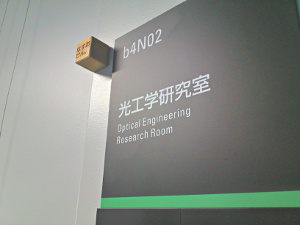
\includegraphics[scale=0.55]{figs/hikari_kogaku}
\caption{
\label{fig:TeNe}
Here is the figure caption.
}
\end{figure*}

%------------------------------------------------------

%\input{tex_files/experiment}
%\input{tex_files/results}

% appendix
%\input{tex_files/appendix_implementation}


\section{Summary}
  Summary comes hrere. bra bra bra


\begin{acknowledgements}
  acknowledgements comes here
  The authors thank bra bra bra

\end{acknowledgements}



\bibliography{refs}
\end{document}
